\section{Mapping rules in spreadsheets: Mapeathor}
\label{sec:chp5_mapeathor}

Since mapping languages started to be used more broadly, there have been multiple approaches for the development of editors to ease their specification. Some of them enable editing through graphical visualization~\citep{heyvaert2016rmleditor,sicilia2017map}, while others provide a writing environment (e.g. the Protégé extension OntopPro~\ana{ref}). Thus, these editors are language-oriented, as they help to create mappings in a specific language. However, use cases require different features and implementations, and as a result, several different mapping languages are used currently. Moreover, graphical interfaces may hinder the mapping management and creation when a large number of mapping rules is required. 

%Moreover, when managing large amounts of mapping rules, graphical interfaces become cumbersome. %With our approach we aim at easing the writing process using a common tool such as spreadsheets, as well as enabling the generation of mapping files in more than one mapping language.

%In our work we focus on facilitating the transformation rule specification using declarative mapping rules. 
This section presents a straightforward approach to create these mapping documents, leveraging the  specification of mapping rules in spreadsheets. These spreadsheets contain the essential elements of the mapping rules without any additional syntax element, and are later translated into one a mapping document. The purpose of this proposal is to increase the interoperability between these languages~\citep{corcho2020towards, iglesias2022devising} as well as to ease the creation process. To perform the mapping rules translation we developed Mapeathor~\citep{iglesias-molina_2023_5973906}, a tool able to parse the spreadsheets and generate the corresponding mappings in R2RML, RML and YARRRML. Following, we present the structure of the spreadsheet to write the mapping rules, the implementation and a evaluation with a user study to validate our approach.

\subsection{Spreadsheet design}
\label{sec:chp5_spreadsheet_design}

%The rules required to generate a knowledge graph can be specified in multiple languages. The language is chosen by the user depending on the specific use case. However, the rules themselves are equivalent across languages, so they can be written in a language-independent way, in this case, we chose a spreadsheet for rule specification. 

In this section we present the design of the spreadsheet template to write the mapping rules. 
These mapping rules are specified in the spreadsheets following a provided structure to only write the essential information. Thus, this approach prevents the user from learning the syntax peculiarities of each languages (e.g. keywords, semicolons, brackets, etc.).
This design is devised to represent the rules in a compact and understandable manner, using a format widely used by the scientific community (i.e. Google spreadsheets, MS Excel). 
Using these spreadsheets along with their corresponding editors allow users to leverage their native advantages.
The mapping rules are specified in the spreadsheet across five different sheets, which are described below: \textit{Prefix sheet}, \textit{Source sheet}, \textit{Subject sheet}, \textit{Predicate\_Object sheet} and \textit{Function sheet}. We illustrate this section with a running example to describe in detail the expressiveness capabilities of each spreadsheet. This example uses the data represented in the CSV file \texttt{people.csv}(\cref{lst:chp5_mapeathor_input_people}) and the JSON file \texttt{sport.json} (\cref{lst:chp5_mapeathor_input_sport}). 

\begin{minipage}{0.48\linewidth}
\begin{captionedlisting}{lst:chp5_mapeathor_input_people}{ Contents of \texttt{people.csv}.}
\centering
\begin{tabular}{c}
%\hspace{1em}
{
\begin{lstlisting}[basicstyle=\ttfamily\small,label={list:example1},columns=flexible]
id , name  , birthdate , sport_id
1  , Emily , 08/02/90  , 2
2  , Jonah , 18/11/75  , 2
\end{lstlisting}
}
\end{tabular}
\end{captionedlisting}
\end{minipage}
\,\,\,\,\hfill
\begin{minipage}{0.52\linewidth}
\begin{captionedlisting}{lst:chp5_mapeathor_input_sport}{Contents of \texttt{sport.csv}.}
\centering
\begin{tabular}{c}
\hspace{1.5em}
{
\begin{lstlisting}[basicstyle=\ttfamily\small,label={list:example1},columns=flexible]
[ {
   "id": 1,
   "sport": " Ice Skating"
 },{
   "id": 2,
   "sport": " Rugby"
 } ]
\end{lstlisting}
}
\end{tabular}
\end{captionedlisting}
\end{minipage}



\ana{poner al final de la sección como traduce o sección a sección; a RML. --$>>$ mejor al final cuando se presente la herramienta, en la siguiente subsección}

\subsubsection{Prefix sheet} 
This sheet contains the namespaces and corresponding prefixes used in the creation of the transformation rules. 
It is composed of two columns: \texttt{Prefix} for the prefix and \texttt{URI} for the corresponding namespace. The base namespace can be specified writing ``@base" in the \texttt{Prefix} column. The namespaces used by the target mapping language are automatically added in the translation (e.g. \texttt{rr}\footnote{\url{http://www.w3.org/ns/r2rml\#}}, \texttt{rml}\footnote{\url{http://semweb.mmlab.be/ns/rml\#}}).
The example shown in \cref{tab:prefix_sheet} presents how three namespaces and the base namespace are written in this template. 

\begin{table}[h!]
\caption{Prefix sheet.}
\label{tab:prefix_sheet}
\centering
\begin{tabular}{c|c}
\midrule
\textbf{Prefix} & \textbf{URI}                                 \\ \midrule
@base           & http://example.com/                          \\
rdf             & http://www.w3.org/1999/02/22-rdf-syntax-ns\# \\
ex              & http://ex.com/                               \\ 
grel            & http://semweb.datasciencelab.be/ns/grel\#     \\
\midrule
\end{tabular}
\end{table}


\subsubsection{Subject sheet} 
This sheet defines how to generate the subjects and a corresponding identifier (\texttt{ID}) that groups the mapping rules per subject. It is organized in four columns: \texttt{ID}, \texttt{URI}, \texttt{Class} and \texttt{Graph}. \texttt{ID} contains a unique identifier for each subject's set of rules in order to relate to information on these rules in the remaining sheets.
\texttt{URI} defines the subject URI of the resources that are to be generated by the mapping. 
\texttt{Class} allows the assignation of the subject to a class with \texttt{rdf:type}. A subject may be type of one class, more than one or none at all. 
Finally, \texttt{Graph} is an optional column that enables the assignation of a named graph to the triples generated for a subject.

The example shown in \cref{tab:subject_sheet} presents how to write two subjects, each with a different identifier and URI for the instances. Within the \texttt{URI} field, what is written between ``\{" and ``\}" references a field in the source data. The instances of the subject with the \texttt{PERSON} ID are type of two classes, (\texttt{ex:Person} and \texttt{ex:Athlete}), while all the triples of the instances of the subject identified with the \texttt{SPORT} ID are assigned to a named graph (\texttt{ex:SportsGraph}). 


\begin{table}[h!]
\caption{Subject sheet.}
\label{tab:subject_sheet}
\centering
\begin{tabular}{c|c|c|c}
\midrule
\textbf{ID} & \textbf{URI} & \textbf{Class} & \textbf{Graph} \\ \midrule
PERSON & http://ex.com/Person/\{name\} & ex:Person &  \\
PERSON & http://ex.com/Person/\{name\} & ex:Athlete &  \\
SPORT & http://ex.com/Sport/\{sport\} & ex:Sport & ex:SportsGraph \\ \midrule
\end{tabular}
\end{table}

\ana{no class}


\subsubsection{Source sheet} 

This sheets describes the source input data for each set of rules, identified with the identifier previously created in the \textit{Subject sheet} (\texttt{ID}). The information is organized in three columns: \texttt{ID}, \texttt{Feature} and \texttt{Value}. 
\texttt{ID} makes reference to the identifier that gathers the mapping rules in the sheets, which was introduced in the \textit{Subject sheet}. 
\texttt{Feature} declares the type of information provided in \texttt{Value}. The allowed keywords in this column are: \texttt{source} for the path and name of the file, \texttt{format} for the data source format, \texttt{iterator} for hierarchical data (e.g. JSON, XML), \texttt{table} for name of tables from Relational Data Bases (RDBs), \texttt{query} for SQL queries and \texttt{SQLVersion} for the version of SQL used. Each ID must have at least the \texttt{source} and \texttt{format} features specified, the rest of the features are optional. 
Then, in the \texttt{Value} column, the corresponding values of each \texttt{Feature} specified are written. 

\cref{tab:source_sheet} shows the data source description for the \texttt{PERSON} and \texttt{SPORT} IDs. The former corresponds to the CSV file shown in \cref{lst:chp5_mapeathor_input_people}, while the latter to the JSON file in \cref{lst:chp5_mapeathor_input_sport}, for which the iterator is also written (\texttt{\$.*}). 

\begin{table}[h!]
\caption{Source sheet.}
\label{tab:source_sheet}
\centering
\begin{tabular}{c|c|c}
\midrule
\textbf{ID} & \textbf{Feature} & \textbf{Value}              \\ \midrule
PERSON    & source          & /home/user/data/people.csv  \\
PERSON    & format          & CSV                         \\
SPORT     & source          & /home/user/data/sports.json \\
SPORT     & format          & JSON                        \\  
SPORT     & iterator        & \$.*                    \\ \midrule
\end{tabular}
\end{table}

\subsubsection{Predicate\_Object sheet} 
This sheet enable users to specify how to generate the triples, that is, predicate-object pairs for the subjects defined in the \textit{Subject sheet}. This sheet contains up to 8 columns: \texttt{ID}, \texttt{Predicate}, \texttt{Object}, \texttt{DataType}, \texttt{Language}, \texttt{ReferenceID}, \texttt{InnerRef} and \texttt{OuterRef}.

The column \texttt{ID} indicates the set of rules which the triples belong to, that has been previously defined in the \textit{Subject} and \textit{Source sheets}.
The columns \texttt{Predicate} and \texttt{Object} specify the predicate and object of the triple respectively. 
The XSD datatype of \texttt{Object} is defined in \texttt{DataType}, and the language tag in \texttt{Language}. Both these columns are optional. 

When the object refers to a subject defined in another mapping rule, the rule is written as follows. 
There are three columns that allow the specification of the linking condition between the object of the current triple and the referenced subject. 
They specify which is the ID of the referred subject  (\texttt{ReferenceID}), and the ''join'' fields in the source data: (i) \texttt{InnerRef} for the field of the object of the current triple, and (ii) \texttt{OuterRef} for the field of the referred subject. These three fields can be blank when a regular triple is produced. 

\cref{tab:po_sheet} shows five predicate-object pairs created for both sets of rules (\texttt{PERSON} and \texttt{SPORT}. Three of these rules produce literals with datatypes and two additionally specify a language tag. The rule set identified as \texttt{PERSON} generates a link to the subject of the \texttt{SPORT} rule set using the predicate \texttt{ex:name}, and joining by equal values of the field \texttt{sport\_id} from \texttt{people.csv} and the field \texttt{id} from \texttt{sport.json}. This rule set also calls a function for generating the object for the predicate \texttt{ex:birthdate}, which is identified by being enclosed by ``$<>$".

\begin{table}[h!]
\caption{Predicate\_Object sheet.}
\label{tab:po_sheet}
\centering
\resizebox{\columnwidth}{!}{
\begin{tabular}{c|c|c|c|c|c|c|c}
\midrule
\textbf{ID} &\textbf{Predicate} & \textbf{Object}               & \textbf{DataType} & \textbf{Language} & \textbf{ReferenceID} & \textbf{InnerRef} & \textbf{OuterRef} \\ \midrule
PERSON & ex:name & \{name\} & string & en & & &  \\
PERSON & ex:birthdate & $<$Fun-date$>$ & & & & & \\
PERSON & ex:plays & & & & SPORT& sport\_id & id \\
SPORT & ex:name & \{sport\} & string & en & & & \\
SPORT & ex:code & \{id\} & integer & & & & \\ \midrule
\end{tabular}
}
\end{table}

\subsubsection{Function sheet} Some languages are able to process data transformation functions, which can be detailed in this sheet. Mapeathor implements the last release of the RML-FNML specification, that describes how to incorporate functions in RML mappings\footnote{\url{https://w3id.org/rml/fnml/spec}}. The functions are referred in the Predicate\_Object sheet or in other function rows with the identifier specified in \texttt{FunctionID}. The column \texttt{Feature} is used to specify the type of information provided in \texttt{Value}. The features admitted in the \texttt{Feature} column are \texttt{executes} for the name of the function, and \texttt{returns} for the expected output type of the function. In addition, this column admits any number of function parameter names. Then, the value of the name of the function, return type and values of the parameters are written correspondingly in the \texttt{Value} column.

The example shown in \cref{tab:function_sheet} uses the function \texttt{grel:toDate}, to change the formatting of a date. It returns a date as output (\texttt{grel:dateOut}) and takes three parameters: the data field to be converted (\texttt{grel:valueParam1}), the input data format (\texttt{grel:valueParam2}) and the output data format (\texttt{grel:valueParam3}).

\begin{table}[h!]
\caption{Function sheet.}
\label{tab:function_sheet}
\centering
\begin{tabular}{c|c|c}
\midrule
\textbf{FunctionID} & \textbf{Feature} & \textbf{Value} \\ \midrule
$<$Fun-date$>$ & executes & grel:toDate \\  
$<$Fun-date$>$ & returns & grel:dateOut \\  
$<$Fun-date$>$ & grel:valueParam1 & \{birthdate\} \\
$<$Fun-date$>$ & grel:valueParam2 & dd/MM/yyyy \\
$<$Fun-date$>$ & grel:valueParam3 & yyyy-MM-dd \\
\midrule
\end{tabular}
\end{table}


\subsection{Mapeathor}
\label{sec:chp5_mapeathor_tool}

Mapeathor~\citep{iglesias-molina_2023_5973906} is a open-source implementation to generate mappings from the spreadsheets described in \cref{sec:chp5_spreadsheet_design}. It is able to process MS Excel and Google Spreadsheets, generating human-readable mappings in either R2RML, RML or YARRRML. 

\textit{descripción de la herramienta, aunque sea de forma sencilla (y se puede poner el diagrama de github). Va a haber que hacer pseudocódigo :)))))}

The source code of Mapeathor is openly available under Apache 2.0 license\footnote{\url{https://github.com/oeg-upm/mapeathor}}. It can be run as a CLI using the Pypi package\footnote{\url{https://pypi.org/project/mapeathor/}} or as an online service\footnote{\url{https://morph.oeg.fi.upm.es/demo/mapeathor}}, where a visual interface is provided. With each release, a new version in Pypi is created and a dedicated DOI archived in Zenodo~\citep{iglesias-molina_2023_5973906}. 


\subsection{Methodology}
\label{sec:chp5_mapeathor_eval_method}

We carry a user study with two dimensions to test the usability of Mapeathor and evaluate if the spreadsheet-based approach can improve the mapping writing process for users of different expertise. We first carry out a \textit{subjective evaluation} in order to gather opinions and feedback about the spreadsheet template and usability of the tool in order to improve the user experience. We then perform a \textit{objective evaluation} to find out if our approach improves the mapping writing process w.r.t. writing directly the mapping in a target language (i.e. RML) and w.r.t. another mapping editor with a visual interface (i.e. RMLEditor). This section describes the methodology followed for the performed evaluations.

%\textit{motivación: qué queremos comprobar, que si facilita la creación de mapping rules para experts y no experts. Para eso llevamos a cabo dos evaluaciones con usuarios, subjectiva y objetiva. En la subjectiva usuarios que han probado el software cuentan su experiencia y opiniones. En la objetiva, cogemos a usuarios y los dividimos en 3 grupos, para que generen mappings con rml, rmleditor y mapeathor. Así vemos si 1) mapeathor mejora RML y si 2) funciona mejor que una herramienta visual. Describir background, que no hay bias porque se puso a gente que nos había utilizado esa tech antes. y resultados}


\noindent\textit{\textbf{Procedure}} The evaluation is comprised of two steps. The first step, correspondent to the \textit{subjective evaluation}, took place during the Knowledge Graph Construction Tutorial co-located with the 19th edition of the Extended Semantic Web Conference (2022)\footnote{\url{https://kg-construct.github.io/eswc-dkg-tutorial-2022/}}. This tutorial hosted a slot for presenting Mapeathor and the spreadsheet design, allowing time for a hands-on exercise at the end of the explanation. At the end of the slot, participants were asked to fill a questionnaire to assess the usability of the approach and gather some feedback for improvements. The questionnaire first inquired about the background of the participants, asking them to rate in a 5-point Likert scale their expertise in (i) linked data and (ii) mapping languages and tools. Then, it assessed the usability of the approach with 10 questions that follow the SUS template, with also a 5-point Likert scale rating; and an additional optional question to gather feedback for improvement (\cref{tab:chp5_sub_questionnaire}).


\begin{table}[t!]
\caption{Questionnaire for subjective assessment of the usability of the spreadsheet design and Mapeathor. }
\centering
\label{tab:chp5_sub_questionnaire}
\resizebox{\columnwidth}{!}
{\begin{tabular}{cl}
\multicolumn{2}{c}{\textbf{Questions}} \\ \midrule
1. & I think that I would like to use this tool frequently\\ \midrule
2. & I found the tool unnecessarily complex\\ \midrule
3. & I thought the spreadsheet template was easy to use\\ \midrule
4. & I think that I would need the support of a technical person to be able to use the spreadsheet template\\ \midrule
5. & I found the different facets in this spreadsheet template were well integrated\\ \midrule
6. & I thought there was too much inconsistency in this tool\\ \midrule
7. & I think that most people would learn how to write the spreadsheet template very quickly\\ \midrule
8. & I found the tool unmanageable to use\\ \midrule
9. & I felt very confident using the spreadsheet template\\ \midrule
10. & I needed to learn a lot of things before I could get going with this tool\\ \midrule
11. & Optional comments (feedback to improve) \\ \bottomrule
\end{tabular}}
\end{table}





The second step of the evaluation that comprises the \textit{objective evaluation} took place in May 2023, once the improvements gathered from the previous step were implemented. In this step, the spreadsheet-based approach proposed in this work was compared with the widely used RML mapping language~\citep{Dimou2014rml}, and with a visual editor, RMLEditor~\citep{heyvaert2016rmleditor}. A group of 30 participants was divided into three groups of 10. Each group had to carry out the same task, to create a mapping from a given dataset and ontology with the assigned tool. All groups were introduced to the needed concepts about mapping languages and specific guidelines with examples of the assigned tool. The groups performed the given task in separated sessions, i.e. one session per tool was carried out, to ensure that all participants were given the same level of assistance independently of the tool. Participants were asked to carry out the proposed task in 30 minutes, after that they were asked to submit the mapping they have created so far. In addition, likewise as in the first step, participants were asked to rate in a 5-point Likert scale their expertise in (i) linked data and (ii) mapping languages and tools; and to write their personal opinion on the assigned tool.


\begin{figure*}[!t]
\centering
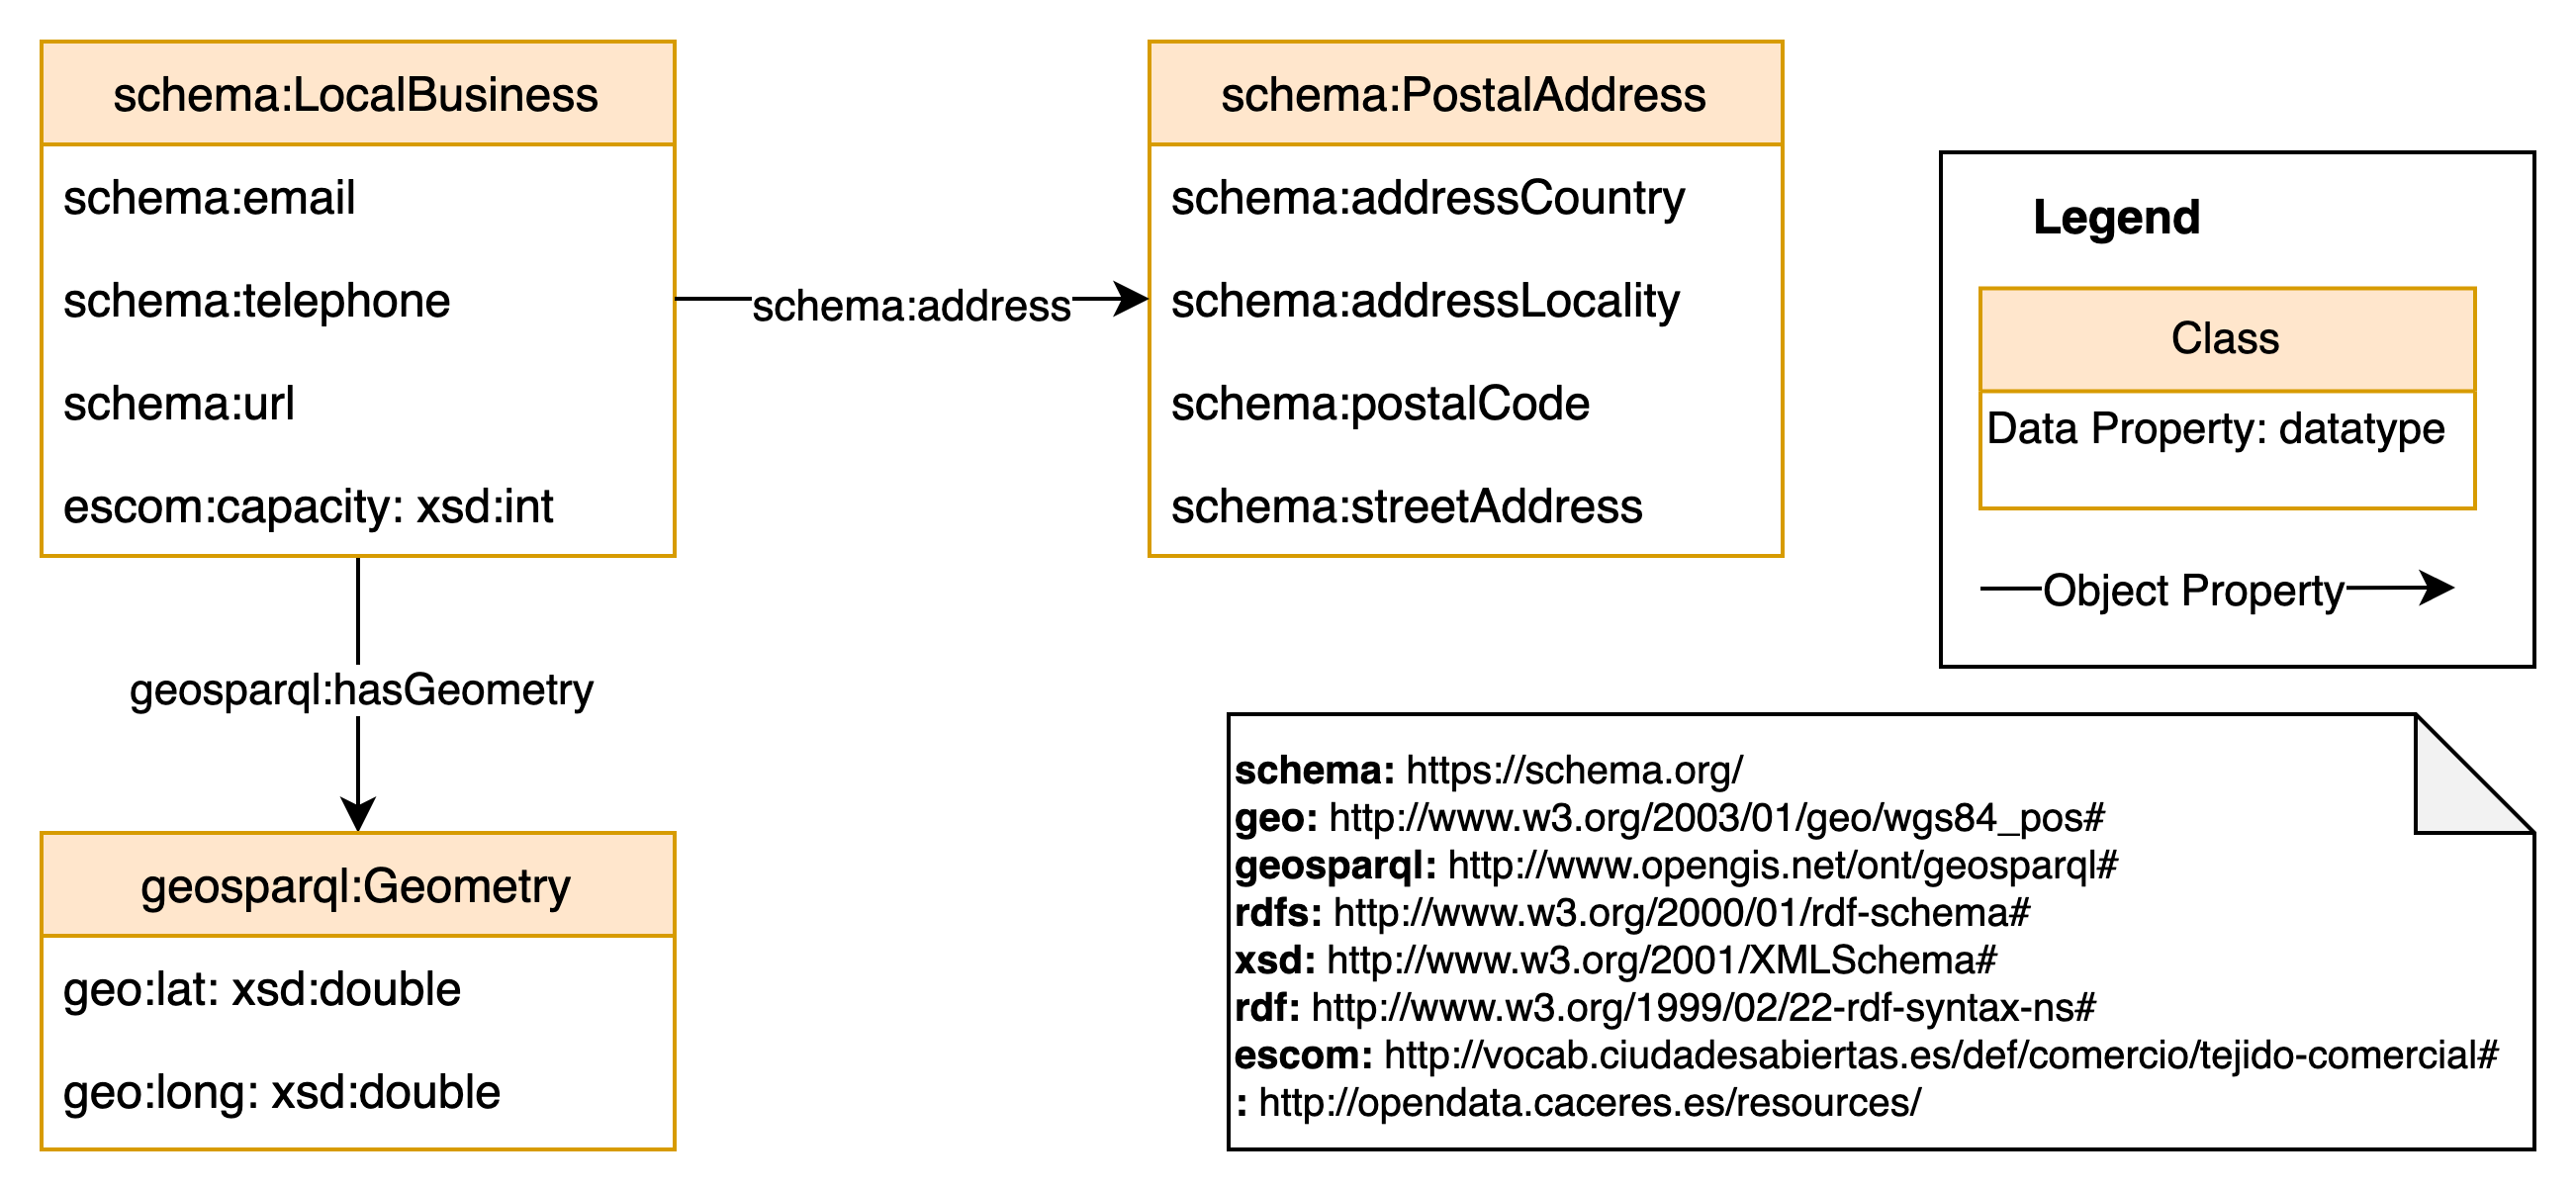
\includegraphics[width=0.85\linewidth]{figures/mapeathor_us_onto.png}
\caption[Ontology diagram for the user study exercise of Mapeathor]{Ontology diagram representing a subset of the Vocabulary for data representation of the local business census and activities licenses.}
\label{fig:chp5_us_onto}
\end{figure*}

\noindent\textit{\textbf{Resources}}
The same data and ontology was used for both evaluations. We use a subset of the \textit{Vocabulary for data representation of the local business census and activities licenses}\footnote{\url{http://vocab.ciudadesabiertas.es/def/comercio/tejido-comercial/index-en.html}} that represents local businesses, their postal address and geolocalization (\cref{fig:chp5_us_onto}). 
We chose this dataset, that belongs to the common-knowledge domain, to avoid heterogeneous prior domain knowledge influence on the results of the study.

We provided participants with the subset ontology description and associated data, that is comprised of three CSV files: \texttt{bar.csv}, \texttt{restaurant.csv} and \texttt{address.csv}. Information about bars, restaurants and their geolocalization is represented in the files \texttt{bar.csv}, \texttt{restaurant.csv} respectively. 
These files contain the same columns, but different data. The file \texttt{address.csv} represent the postal address of the businesses present in the other two files. 
The original data is available in GitHub\footnote{\url{https://github.com/CiudadesAbiertas/vocab-comercio-censo-locales/}}. 
To facilitate the exercise for participants, some data cleaning was performed over the original files, as well as translation to all columns form spanish to english~\citep{iglesias-molina_2022_8154522}.



\noindent\textit{\textbf{Participants}} 
In the \textit{subjective evaluation}, 17 attendants submitted answers to the questionnaire provided during the session. Most of the participants were knowledgeable in linked data, while less than half had already used mappings before. 
In the \textit{objective evaluation}, 30 participants were sampled from the Ontology Engineering Group, ranging from MSc students to full professors. Their background ranged from having basic knowledge about linked data and mappings, to being knowledgeable practitioners, including participants that were experts in linked data but had no knowledge about mappings. Participants were pseudo-randomly divided into three groups, one per tool. Prior to this assignation, participants were asked to provide information about whether they had prior knowledge of any of the tools, so that no participant would use a tool which they were already familiar with. Each group was balanced w.r.t. the heterogeneity in background. 

\noindent\textit{\textbf{Metrics}} 
The \textit{subjective evaluation} measured the responses to the SUS questionnaire on a 5-point Likert scale. 
For the \textit{objective evaluation},
%the accuracy of the mapping submitted was calculated. All participants had 30 minutes to perform the task and upload the resulting mapping, thus two kinds of accuracies are calculated. \ana{igual esta frase cuadrarla después }
we calculate two kinds of accuracies: (i)~\textit{Total Accuracy} (TA) for the number of correct rules written w.r.t. the reference correct mapping, and (ii)~\textit{Local Accuracy} (LA) for the number of correct rules w.r.t. all the rules written. We calculate both accuracies because of the fixed time for completing the exercise. TA can be interpreted as a measure of completeness, while LA focusses on assessing the correctness of the written rules independently on the total completeness.
We divide the mapping in four components: \textit{Subject}, \textit{Source}, \textit{Predicate-Object (PO)} and \textit{Join}, and calculate the accuracy for each component and the totality of the mapping. Then a T-Test is performed to look for significant differences of accuracy among the tools. 


\noindent\textit{\textbf{Threats to validity}}~\citep{creswell2017research} We identify the following internal and external threats to the validity of our experiment.

\textbf{Internal validity threats} concern the experimental setup or experience of participants which threaten the ability to draw correct conclusions about the population in the experiment. We identify three internal threats: \textit{tool familiarity bias}, \textit{selection bias} and \textit{instruction bias}.
\begin{itemize}
    \item \textbf{Tool familiarity bias.} Practitioners tend to be more expert in some specific technologies and languages that they use more frequently. Thus, in the sample there it is possible to have participants that have used any of the tested approaches, which in turn can influence the results. For creating the groups, participants' experience was inquired to avoid assigning them a tool that they had previously used.
    \item \textbf{Selection bias.} The sample includes participants with different range on skills and previous knowledge about linked data and mappings. We mitigate this threat by defining groups that were  homogeneous w.r.t. range of expertise in mappings and linked data, considering also the mitigation measures for the \textit{tool familiarity} threat. That is to say, all groups included from beginner users to knowledgeable practitioners. 
    \item \textbf{Instruction bias.} One of the evaluated approaches is designed by the conductors of the user study. This situation could incur in bias on information delivery. To mitigate this threat, we provided participants with the same instruction guidelines for each tool. Three sessions were conducted subsequently to provide the same explanations and attention to each tool. During each sessions, all questions were answered with equal level of detail and guidance for all tools and participants.
\end{itemize}

\textbf{External validity threats} occur when wrong inferences from sample data are made beyond the studied sample or experimental setup. We identify two external threats: \textit{background of participants sample} and \textit{environment}.
\begin{itemize}
    \item \textbf{Background of participants sample.} This threat concerns the generalization to individuals outside the study. The sample of participants include a wide range in the variety of backgrounds, from not very familiar with linked data and mappings, to experts. We deliberately choose to have this variety for each group so that the results can be generalized to a broader sample, while mitigating the risks of internal threats described above that this choice poses. 
    \item \textbf{Environment.} This threat concerns the generalization to individuals outside the experiment’s setting. Participants were free to use a computer, browser and tools of their choice. Thus, they could perform the tasks required for the study in a well-known environment. No specific experimental setup prevents generalizations to individuals outside our study.
\end{itemize}




\subsection{Results}
\label{sec:chp5_mapeathor_results}

\noindent\textit{\textbf{Subjective evaluation results}}

\noindent\textit{\textbf{Objective evaluation results}}

\ana{gráficas background per group and general}
\begin{table}[h]
\caption{Results of the user study, showing the mean of the local accuracy (LA), total accuracy (TA) and p-value of the submitted responses per mapping feature and tool.}
\label{tab:chp5_summary_mapeathor}
\centering
\resizebox{\columnwidth}{!}
{\begin{tabular}{ccc|cc|cc|cc|cc}
    \cmidrule{2-11}
    & \multicolumn{2}{c|}{\textbf{Subject}} & \multicolumn{2}{c|}{\textbf{Source}} & \multicolumn{2}{c|}{\textbf{POM}} & \multicolumn{2}{c|}{\textbf{Join}} & \multicolumn{2}{c}{\textbf{Total}} \\ \cmidrule{2-11}
    & LA & TA & LA & TA & LA & TA & LA & TA & LA & TA \\ \midrule
    \textbf{\makecell{RML}} & 0.617 & 0.457 & 0.927 & 0.570 & \underline{0.684} & 0.458 & \underline{0.133} & \underline{0.150} & \underline{0.693} & 0.410  \\ \midrule
    \textbf{\makecell{RMLEditor}} & \underline{0.465} & \underline{0.360} & \underline{0.860} & \underline{0.560} & 0.705 & \underline{0.363} & 0.233 & 0.217 & 0.705 & \underline{0.340}  \\ \midrule
    \textbf{Mapeathor} & \textbf{0.858} & \textbf{0.620} & \textbf{0.960} & \textbf{0.620} & \textbf{0.795} & \textbf{0.581} & \textbf{0.250} & \textbf{0.225} & \textbf{0.831} & \textbf{0.547}  \\\midrule \midrule
    \textbf{p-value} & 0.090 & 0.295 & 0.596 & 0.890 & 0.777 & 0.337 & 0.746 & 0.881 & 0.476 &  0.264 \\ \bottomrule
\end{tabular}}
\end{table}



\begin{figure}[t!]
    \centering
    \begin{subfigure}[b]{\linewidth}
    	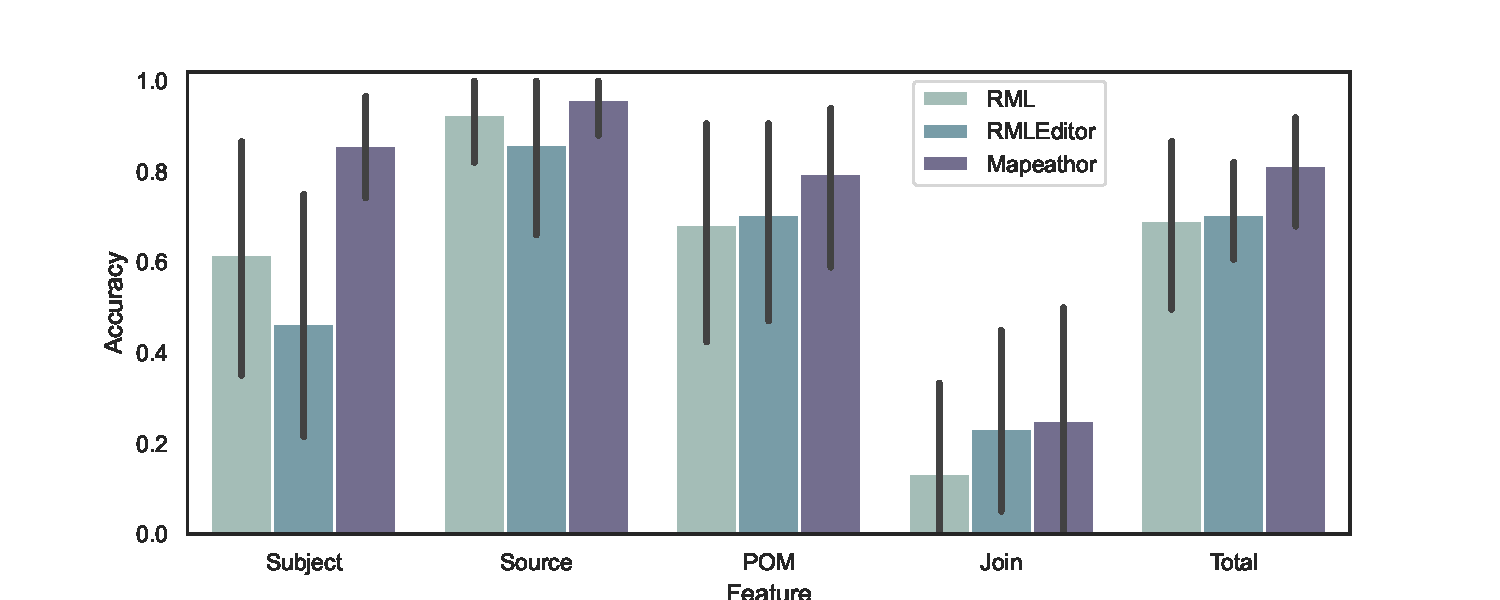
\includegraphics[width=\linewidth]{figures/mapeathor_rel-acc.pdf}
    	\caption{Local accuracy.}
    	\label{fig:chp5_mapeathor_relacc}
    \end{subfigure}
    %\hspace{0.05\textwidth}
    \begin{subfigure}[b]{\linewidth}
    	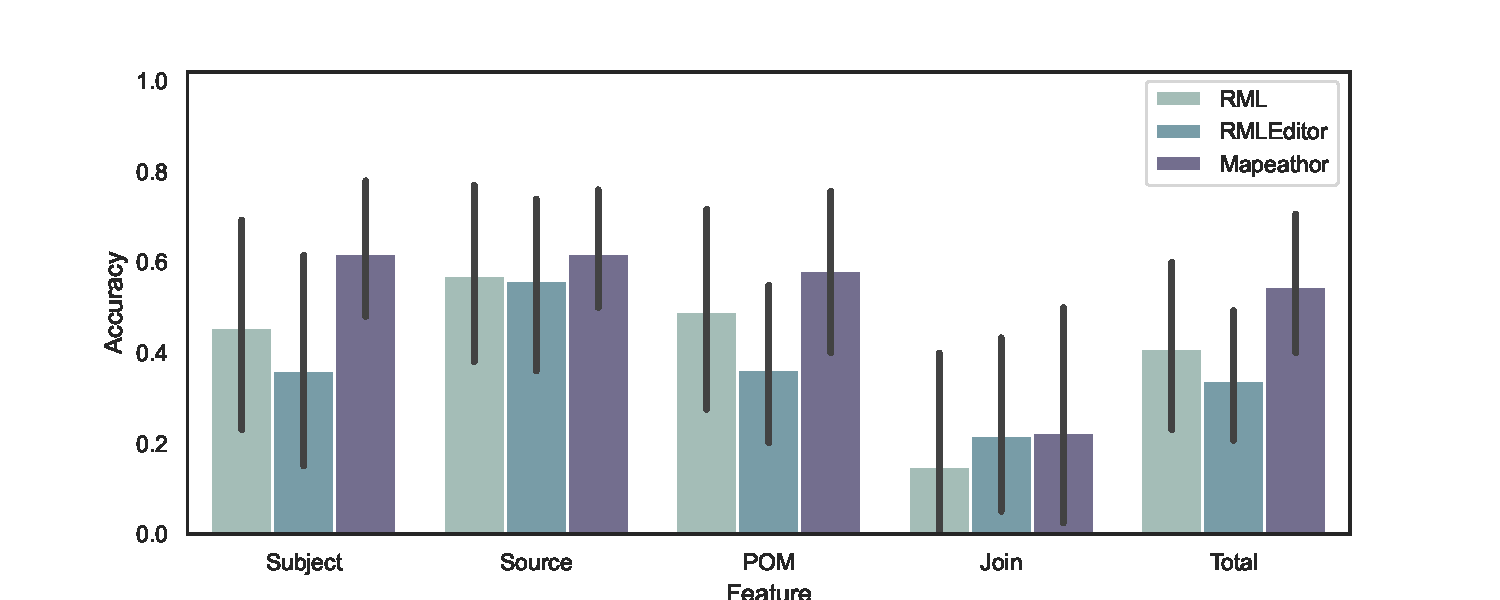
\includegraphics[width=\linewidth]{figures/mapeathor_total-acc.pdf}
    	\caption{Total accuracy.}
    	\label{fig:chp5_mapeathor_totacc}
    \end{subfigure}
    \caption{Accuracy results.}
    \label{fig:reification-app}
\end{figure}


\subsection{Use cases}
Ciudades abiertas, EBOCA, photocatalisis ontology
\ana{bueno ya veremos}



\subsection{Discussion}
\label{sec:chp5_mapeathor_discussion}

\ana{newpage hasta que la seccióne esté entera, borrar después}
\newpage